\section{Misura di alcune resistenze}
\subsection{Montaggio del circuito con resistenza R e acquisizione dati}
Per prima cosa abbiamo ordinato le resistenze controllando i vari valori nominali indicati dalle usuali barre colorate.
Fatto ciò, abbiamo utilizzato il multimetro digitale per misurare il valore esatto di resistenza. Come ci si aspettava, tali valori erano compatibili entro l'incertezza fornita dal costruttore con i valori nominali.
Si è passati dunque a montare il circuito. Ricordiamo che sono state sfruttate le bocchette della breadboard per collegare la resistenza al circuito. Così facendo, è stato assicurato un buon contatto con i cavi principali (evitando così che accidentalmente potesse staccarsi nel momento in cui trafficavamo con il cablaggio).
Sapendo che vi era necessità di cambiare spesso configurazione tra "amperometro a monte" e "amperometro a valle", abbiamo sistemato i cavi in modo che bastasse spostare un solo contatto per cambiare la posizione circuitale dell'amperometro. In Figura \ref{fig:circuiti} sono riportati gli schemi circuitali delle due configurazioni.

Prima di procedere all'acquisizione dati, abbiamo calcolato il valore massimo di tensione applicabile al circuito. Infatti, le resistenze da noi utilizzate sopportavano una potenza massima prima di bruciarsi che variava da $0.1W$ per le più piccole a $0.5W$ per le più grandi. Utilizzando la legge di $Joule$, $P=\frac{V^2}{R}$ e invertendola, abbiamo ottenuto la $V_{MAX}$ applicabile. % avevi scritto 0.5W per entrambe le resistenze, qual è il valore corretto?
Abbiamo dunque chiuso il circuito e annotati i valori di tensione e corrente forniti dai due tester ICE. Ricordiamo che per evitare di rovinare i fragili strumenti abbiamo sempre lasciato il tester usato per misurare correnti sulla scala $5A$, cambiando poi scala progressivamente facendo attenzione a non uscire dal $range$. E' importante ricordare che l'incertezza sul valore letto è $\frac{1}{50}$ del fondo-scala utilizzato. Per questo motivo si è sempre cercato di mantenere la lancetta dello strumento oltre la metà del quadrante graduato. Come si vedrà tratterà nelle conclusioni, non sempre è stato possibile fare ciò. Abbiamo provato a valutare l'errore statistico su una singola misura aprendo e chiudendo il circuito. Si è subito notato che il valore riportato dagli strumenti rimaneva invariato, indice che la precisione dello strumento non ci permetteva di apprezzare l'errore statistico.

\subsection{Analisi dati}

Abbiamo calcolato il valore delle resistenze applicando semplicemente l'equazione $R_m=\frac{V_m}{I_m}$. Si è notata subito una notevole differenza con i valori misurati dal multimetro digitale. Tale discrepanza è dovuta alle resistenze interne al voltmetro e all'amperometro che ne distubano la misura. Questo problema è stato risolto considerando il circuito con gli strumenti di misura non ideali. Dunque, utilizzando le equazioni di Kirchhoff, abbiamo calcolato i valori di $R$ in funzione delle resistenze interne degli strumenti di misura e dei valori di corrente e tensione misurati. Le relazioni da noi ottenute sono:
\begin{multicols}{2}
%
\begin{equation}
R=\frac{R_VV}{V-IR_V}
\label{casapagliaccio}
\end{equation}
\begin{equation}
R=\frac{V}{I}-R_A
\label{brugnagay}
\end{equation}

\end{multicols} 

dove l'equazione (\ref{casapagliaccio}) è riferita al circuito (a) mentre l'equazione (\ref{brugnagay}) relativa ad (b). Abbiamo indicato con $R_V$ e $R_A$ le resistenze interne degli strumenti utilizzati. 
Ricordiamo che per calcolare i valori $R_V$ e $R_A$ sono stati risolti i circuiti interni degli strumenti stessi, forniti dal produttore. 

Riportiamo ora il grafico delle resistenze, misurate tramite multimetro digitale e tester ICE. 

\begin{figure}[h]
    \centering
        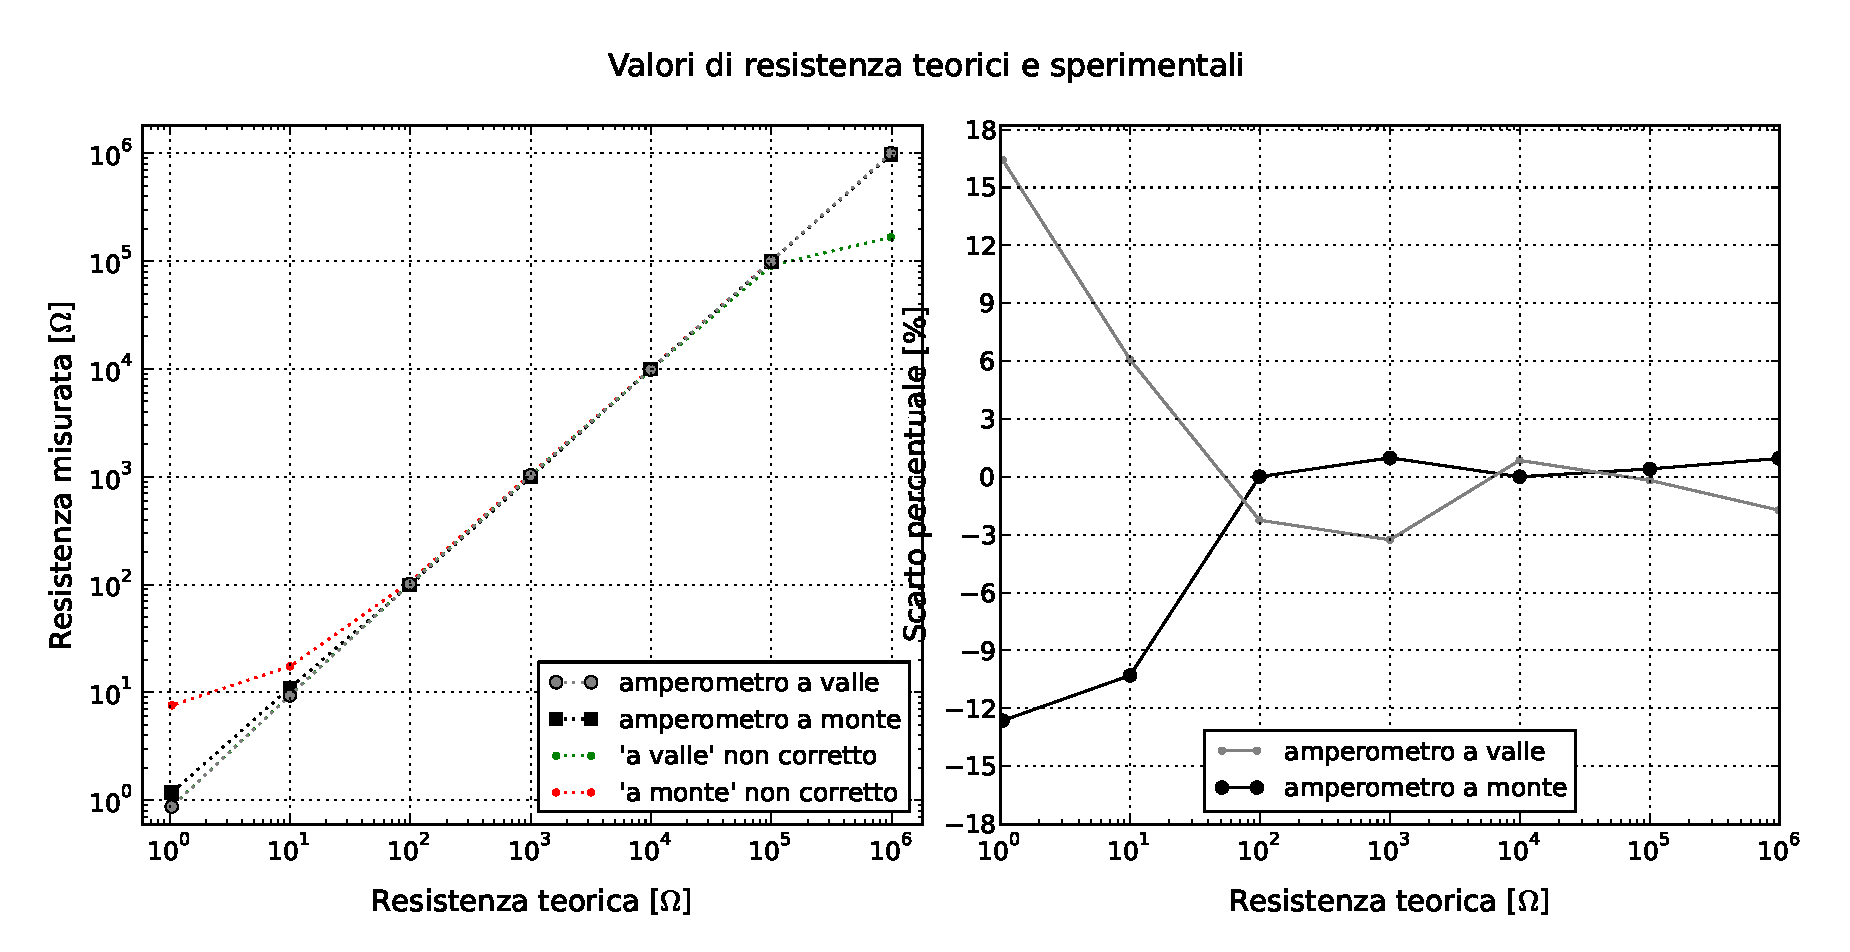
\includegraphics[width=\textwidth]{Res.eps}%{Res_70.eps}
        \caption{Il primo grafico mostra i valori sperimentali delle resistenze, sia corretti con le resistenze interne degli strumenti di misura che senza tale correzione, in funzione dei valori teorici delle resistenze. Si noti che il grafico ha entrambi gli assi in scala logaritmica. Il secondo grafico mostra invece gli scarti in percentuale tra il valore teorico delle resistenze e quello sperimentale. In questo grafico solo la scala sull'asse delle ascisse è logaritmica.}
        \label{fig:resistenze}
\end{figure}

